\section{Les commandes de vol}
	\subsection{Les axes}
	Un aéronef peut bouger sur 3 axes :
	\begin{itemize}
		\item l'axe du roulis \anglais{roll} : il s'agit de l'axe gauche-droite. Cet axe se pilote via les ailerons qui sont actionnés via des mouvements latéraux du manche.
		\item l'axe du tangage \anglais{pitch} : il s'agit de l'axe avant arrière. Cet axe se pilote grâce à la gouverne de profondeur, actionnée via les mouvements longitudinaux du manche. 
		\item l'axe du lacet \anglais{yaw} : il s'agit de l'axe latéral. Cet axe se pilote grâce au gouvernail, actionné grâce aux palonniers.
	\end{itemize}
	
	\begin{figure}[H]
  		\centering
    		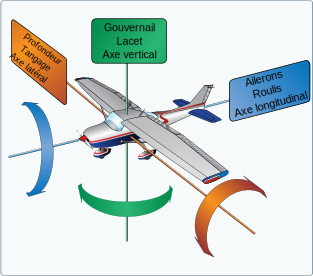
\includegraphics[width=0.6\textwidth]{01-EtudeAeronefs/img/axes.pdf}
  		\legende{Les 3 axes d'un aéronef}{img:axes}
	\end{figure}	
	
	\histoire{On doit à Robert Esnault-Pelterie, ingénieur français, l'invention des ailerons (1905) et du manche à ballet (1906).}
	
	\subsection{Contrôle en roulis}
	Le pilotage en roulis est principalement réalisé grâce à une action sur les ailerons.
	
	Lorsque le pilote actionne le manche d'un côté, l'aileron de l'aile du côté ou le manche est incliné monte, tandis que l'aileron opposé descend. Cela provoque une dissymétrie de portance : la portance augmente du côté ou l'aileron est baissé (même principe qu'un volet), tandis que la portance sur l'aile opposée diminue. En conséquence l'aile avec la surplus de portance monte et la l'aile opposée descend.
	
	\begin{figure}[H]
  		\centering
    		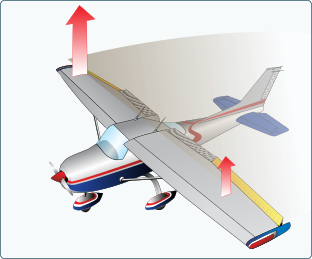
\includegraphics[width=0.6\textwidth]{01-EtudeAeronefs/img/virage.pdf}
  		\legende{Principe de mise en virage par action sur les ailerons}{img:virage}
	\end{figure}	
	
	\subsubsection{Le lacet inverse}
		\begin{figure}[H]
			\centering
  			\includegraphics[width=0.6\textwidth]{01-EtudeAeronefs/img/lacetInverse.pdf}
  			\legende{Lacet inverse (à droite pour un virage à gauche)}{img:lacetInverse}	
		\end{figure}	
	
	\subsection{Contrôle en tangage}
		\begin{figure}[H]
			\centering
  			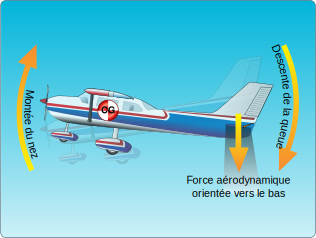
\includegraphics[width=0.6\textwidth]{01-EtudeAeronefs/img/gouverneProfondeur.pdf}
  			\legende{Commande de profondeur}{img:gouverneProfondeur}	
		\end{figure}
		
	\subsection{Le contrôle en lacet}
		\begin{figure}[H]
			\centering
  			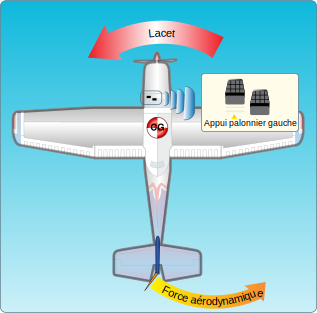
\includegraphics[width=0.6\textwidth]{01-EtudeAeronefs/img/gouverneDeDirection.pdf}
  			\legende{Commande de profondeur}{img:gouverneDeDirection}	
		\end{figure}	
		
		\subsubsection{Le roulis induit}